\documentclass{article}
\usepackage{graphicx}

\begin{document}

\title{The White Whale}
\author{Herman Melville}
\maketitle

\section*{The Captain}

 But as the strange captain, leaning over the pallid bulwarks, was in the act of putting his trumpet to his mouth, it somehow fell from his hand into the sea; and the wind now rising amain, he in vain strove to make himself heard without it. Meantime his ship was still increasing the distance between. While in various silent ways the seamen of the Pequod were evincing their observance of this ominous incident at the first mere mention of the White Whale's name to another ship, Ahab for a moment paused; it almost seemed as though he would have lowered a boat to board the stranger, had not the threatening wind forbade. But taking advantage of his windward position, he again seized his trumpet, and knowing by her aspect that the stranger vessel was a Nantucketer and shortly bound home, he loudly hailed -- 'Ahoy there! This is the Pequod, bound round the world! Tell them to address all future letters to the Pacific ocean! and this time three years, if I am not at home, tell them to address them to -- -- '

\section{More on the Ocean}

   At that moment the two wakes were fairly crossed, and instantly, then, in accordance with their singular ways, shoals of small harmless fish, that for some days before had been placidly swimming by our side, darted away with what seemed shuddering fins, and ranged themselves fore and aft with the stranger's flanks. Though in the course of his continual voyagings Ahab must often before have noticed a similar sight, yet, to any monomaniac man, the veriest trifles capriciously carry meanings. 

Now, how had this noble rescue been accomplished? Why, diving after the slowly descending head, Queequeg with his keen sword had made side lunges near its bottom, so as to scuttle a large hole there; then dropping his sword, had thrust his long arm far inwards and upwards, and so hauled out our poor Tash by the head. He averred, that upon first thrusting in for him, a leg was presented; but well knowing that that was not as it ought to be, and might occasion great trouble; -- he had thrust back the leg, and by a dexterous heave and toss, had wrought a somerset upon the Indian; so that with the next trial, he came forth in the good old way -- head foremost. As for the great head itself, that was doing as well as could be expected.

   And thus, through the courage and great skill in obstetrics of Queequeg, the deliverance, or rather, delivery of Tashtego, was successfully accomplished, in the teeth, too, of the most untoward and apparently hopeless impediments; which is a lesson by no means to be forgotten. Midwifery should be taught in the same course with fencing and boxing, riding and rowing.

   I know that this queer adventure of the Gay-Header's will be sure to seem incredible to some landsmen, though they themselves may have either seen or heard of some one's falling into a cistern ashore; an accident which not seldom happens, and with much less reason too than the Indian's, considering the exceeding slipperiness of the curb of the Sperm Whale's well.

\begin{figure}[!htp]
  \begin{center}
      \includegraphics{whale-8546-svg}
    \caption{
        \textbf{Sperm whale}
        A sperm whale, in svg.
    }
  \end{center}
\end{figure}

   But, peradventure, it may be sagaciously urged, how is this? We thought the tissued, infiltrated head of the Sperm Whale, was the lightest and most corky part about him; and yet thou makest it sink in an element of a far greater specific gravity than itself. We have thee there. Not at all, but I have ye; for at the time poor Tash fell in, the case had been nearly emptied of its lighter contents, leaving little but the dense tendinous wall of the well -- a double welded, hammered substance, as I have before said, much heavier than the sea water, and a lump of which sinks in it like lead almost. But the tendency to rapid sinking in this substance was in the present instance materially counteracted by the other parts of the head remaining undetached from it, so that it sank very slowly and deliberately indeed, affording Queequeg a fair chance for performing his agile 
   obstetrics on the run, as you may say. Yes, it was a running delivery, so it was.

      Now, had Tashtego perished in that head, it had been a very precious perishing; smothered in the very whitest and daintiest of fragrant spermaceti; coffined, hearsed, and tombed in the secret inner chamber and sanctum sanctorum of the whale. Only one sweeter end can readily be recalled -- the delicious death of an Ohio honey-hunter, who seeking honey in the crotch of a hollow tree, found such exceeding store of it, that leaning too far over, it sucked him in, so that he died embalmed. How many, think ye, have likewise fallen into Plato's honey head, and sweetly perished there? 


 When gliding by the Bashee isles we emerged at last upon the great South Sea; were it not for other things, I could have greeted my dear Pacific with uncounted thanks, for now the long supplication of my youth was answered; that serene ocean rolled eastwards from me a thousand leagues of blue.

\begin{figure}[!htp]
  \begin{center}
      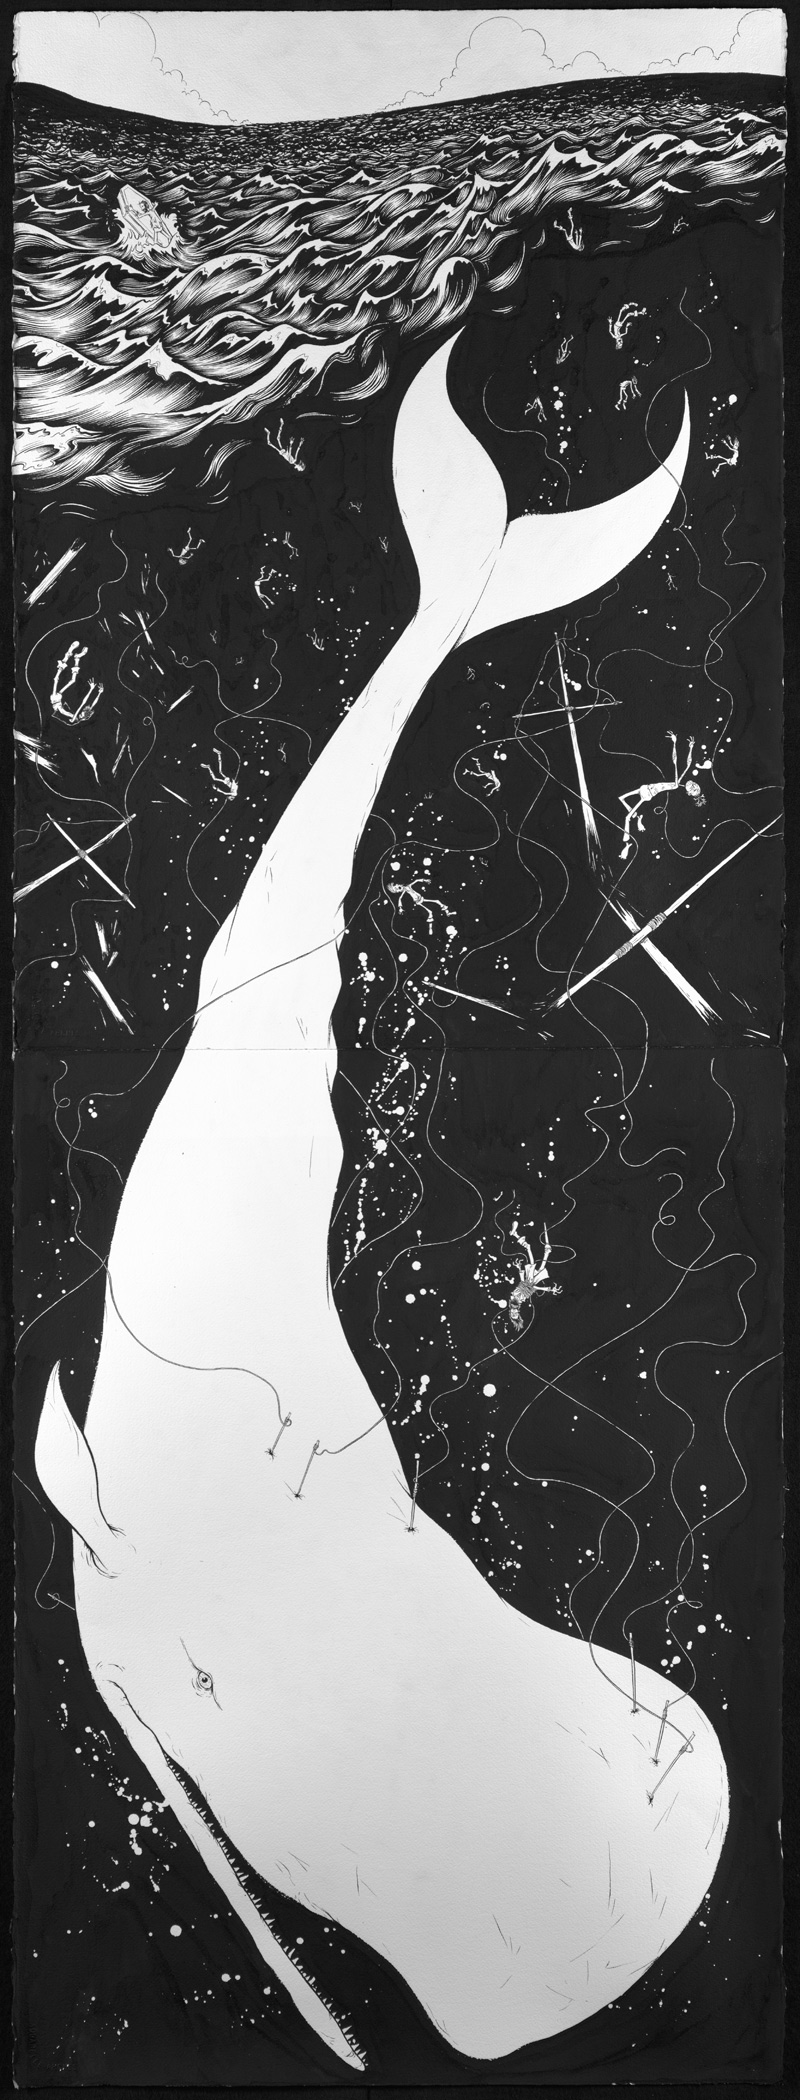
\includegraphics{moby_dick_11}
    \caption{
        \textbf{Moby Dick, or, the Whale.}
My soul is more than matched; she's overmanned; and by a madman! Insufferable sting, that sanity should ground arms on such a field! But he drilled deep down, and blasted all my reason out of me! I think I see his impious end; but feel that I must help him to it. Will I, nill I, the ineffable thing has tied me to him; tows me with a cable I have no knife to cut. Horrible old man! Who's over him, he cries;—aye, he would be a democrat to all above; look, how he lords it over all below! Oh! I plainly see my miserable office,—to obey, rebelling; and worse yet, to hate with touch of pity! For in his eyes I read some lurid woe would shrivel me up, had I it. Yet is there hope. Time and tide flow wide. The hated whale has the round watery world to swim in, as the small gold-fish has its glassy globe. His heaven-insulting purpose, God may wedge aside. I would up heart, were it not like lead. But my whole clock's run down; my heart the all-controlling weight, I have no key to lift again. 
    }
  \end{center}
\end{figure}

   There is, one knows not what sweet mystery about this sea, whose gently awful stirrings seem to speak of some hidden soul beneath; like those fabled undulations of the Ephesian sod over the buried Evangelist St. John. And meet it is, that over these sea- pastures, wide-rolling watery prairies and Potters' Fields of all four continents, the waves should rise and fall, and ebb and flow unceasingly; for here, millions of mixed shades and shadows, drowned dreams, somnambulisms, reveries; all that we call lives and souls, lie dreaming, dreaming, still; tossing like slumberers in their beds; the ever-rolling waves but made so by their restlessness.

   To any meditative Magian rover, this serene Pacific, once beheld, must ever after be the sea of his adoption. It rolls the midmost waters of the world, the Indian ocean and Atlantic being but its arms. The same waves wash the moles of the new-built Californian towns, but yesterday planted by the recentest race of men, and lave the faded but still gorgeous skirts of Asiatic lands, older than Abraham; while all between float milky-ways of coral isles, and low-lying, endless, unknown Archipelagoes, and impenetrable Japans. Thus this mysterious, divine Pacific zones the world's whole bulk about; makes all coasts one bay to it; seems the tide-beating heart of earth. Lifted by those eternal swells, you needs must own the seductive god, bowing your head to Pan.

   But few thoughts of Pan stirred Ahab's brain, as standing like an iron statue at his accustomed place beside the mizen
rigging, with one nostril he unthinkingly snuffed the sugary musk from the Bashee isles (in whose sweet woods mild lovers must be walking), and with the other consciously inhaled the salt breath of the new found sea; that sea in which the hated White Whale must even then be swimming. Launched at length upon these almost final waters, and gliding towards the Japanese cruising-ground, the old man's purpose intensified itself. His firm lips met like the lips of a vice; the Delta of his forehead's veins swelled like overladen brooks; in his very sleep, his ringing cry ran through the vaulted hull, Stern all! the White Whale spouts thick blood! 

\end{document}
